%%%%%%%%%%%%%%%%%%%%%%%%%%%%%%%%%%%%
% Appendix A, Solution and Estimation Details
%%%%%%%%%%%%%%%%%%%%%%%%%%%%%%%%%%%%

% Set equation, figure, table indexing
\renewcommand{\thefigure}{A.\arabic{figure}}
\setcounter{figure}{0}
\renewcommand{\thetable}{A.\arabic{table}}
\setcounter{table}{0}
\renewcommand{\theequation}{A.\arabic{equation}}
\setcounter{equation}{0}
\renewcommand{\thefootnote}{A.\arabic{footnote}}
\setcounter{footnote}{0}

\section{Data} % (fold)
\label{sec:data-ap}

\begin{figure}[H]
\centering
\caption{Examples of an Implicit Association Test}
\label{fig:iatexamples}
\begin{subfigure}{.48\textwidth}
\centering
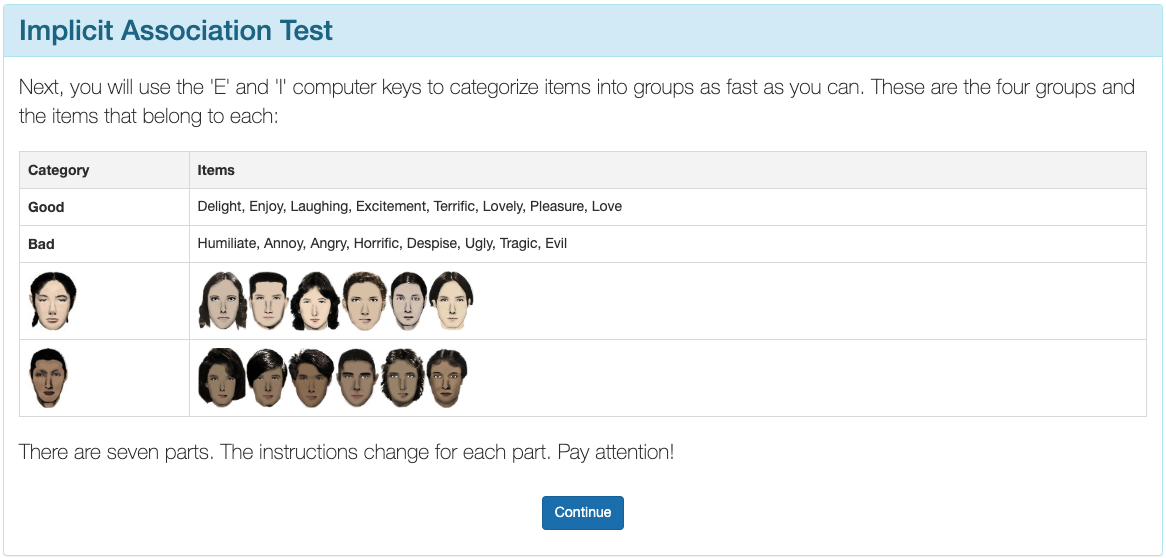
\includegraphics[width=.9\linewidth]{figure/iatexample1.png}
\end{subfigure}
\centering
%Second graph
\begin{subfigure}{.48\textwidth}
\centering
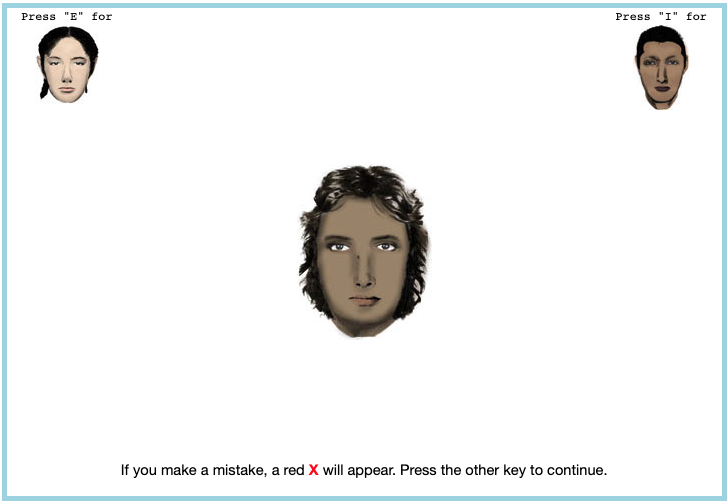
\includegraphics[width=.9\linewidth]{figure/iatexample2.png}
\end{subfigure}
%Third
\begin{subfigure}{.48\textwidth}
\centering
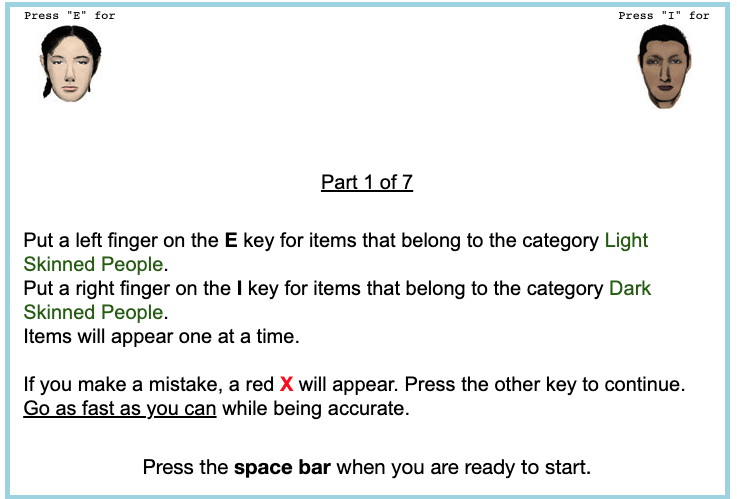
\includegraphics[width=.9\linewidth]{figure/iatexample3.png}
\end{subfigure}
% Fourth
\begin{subfigure}{.48\textwidth}
\centering
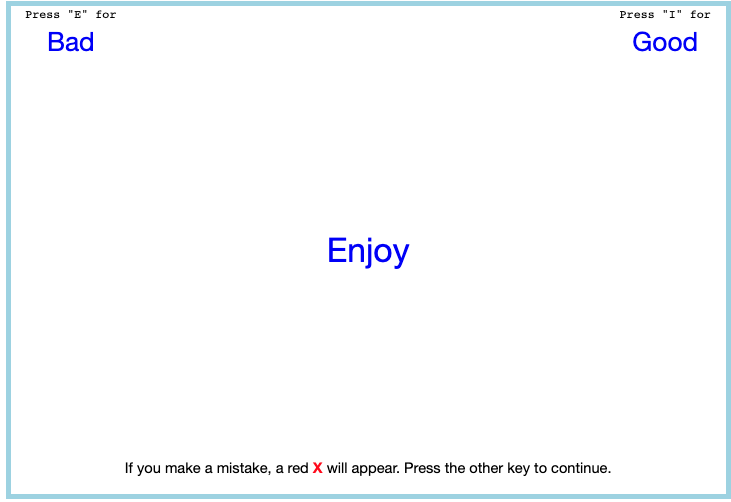
\includegraphics[width=.9\linewidth]{figure/iatexample4.png}
\end{subfigure}
%Fifth
\begin{subfigure}{.48\textwidth}
\centering
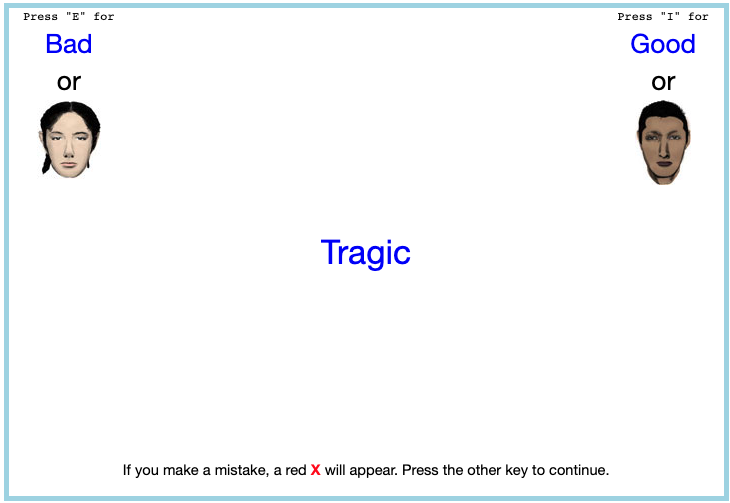
\includegraphics[width=.9\linewidth]{figure/iatexample5.png}
\end{subfigure}
\caption*{\footnotesize{Here are a few examples of what a respondent would see on an implicit association test.}}
\end{figure}

\newpage
\pagebreak

\section{Figures}\label{appendix:figs}

\begin{figure}[H]
    \centering
    \caption{Scatter Plot of Proportion Subjectively Asian on Bias}
    \label{scatter-plot-1}
    \begin{subfigure}{.9\textwidth}
    \caption{Year < 2015}
    \centering
    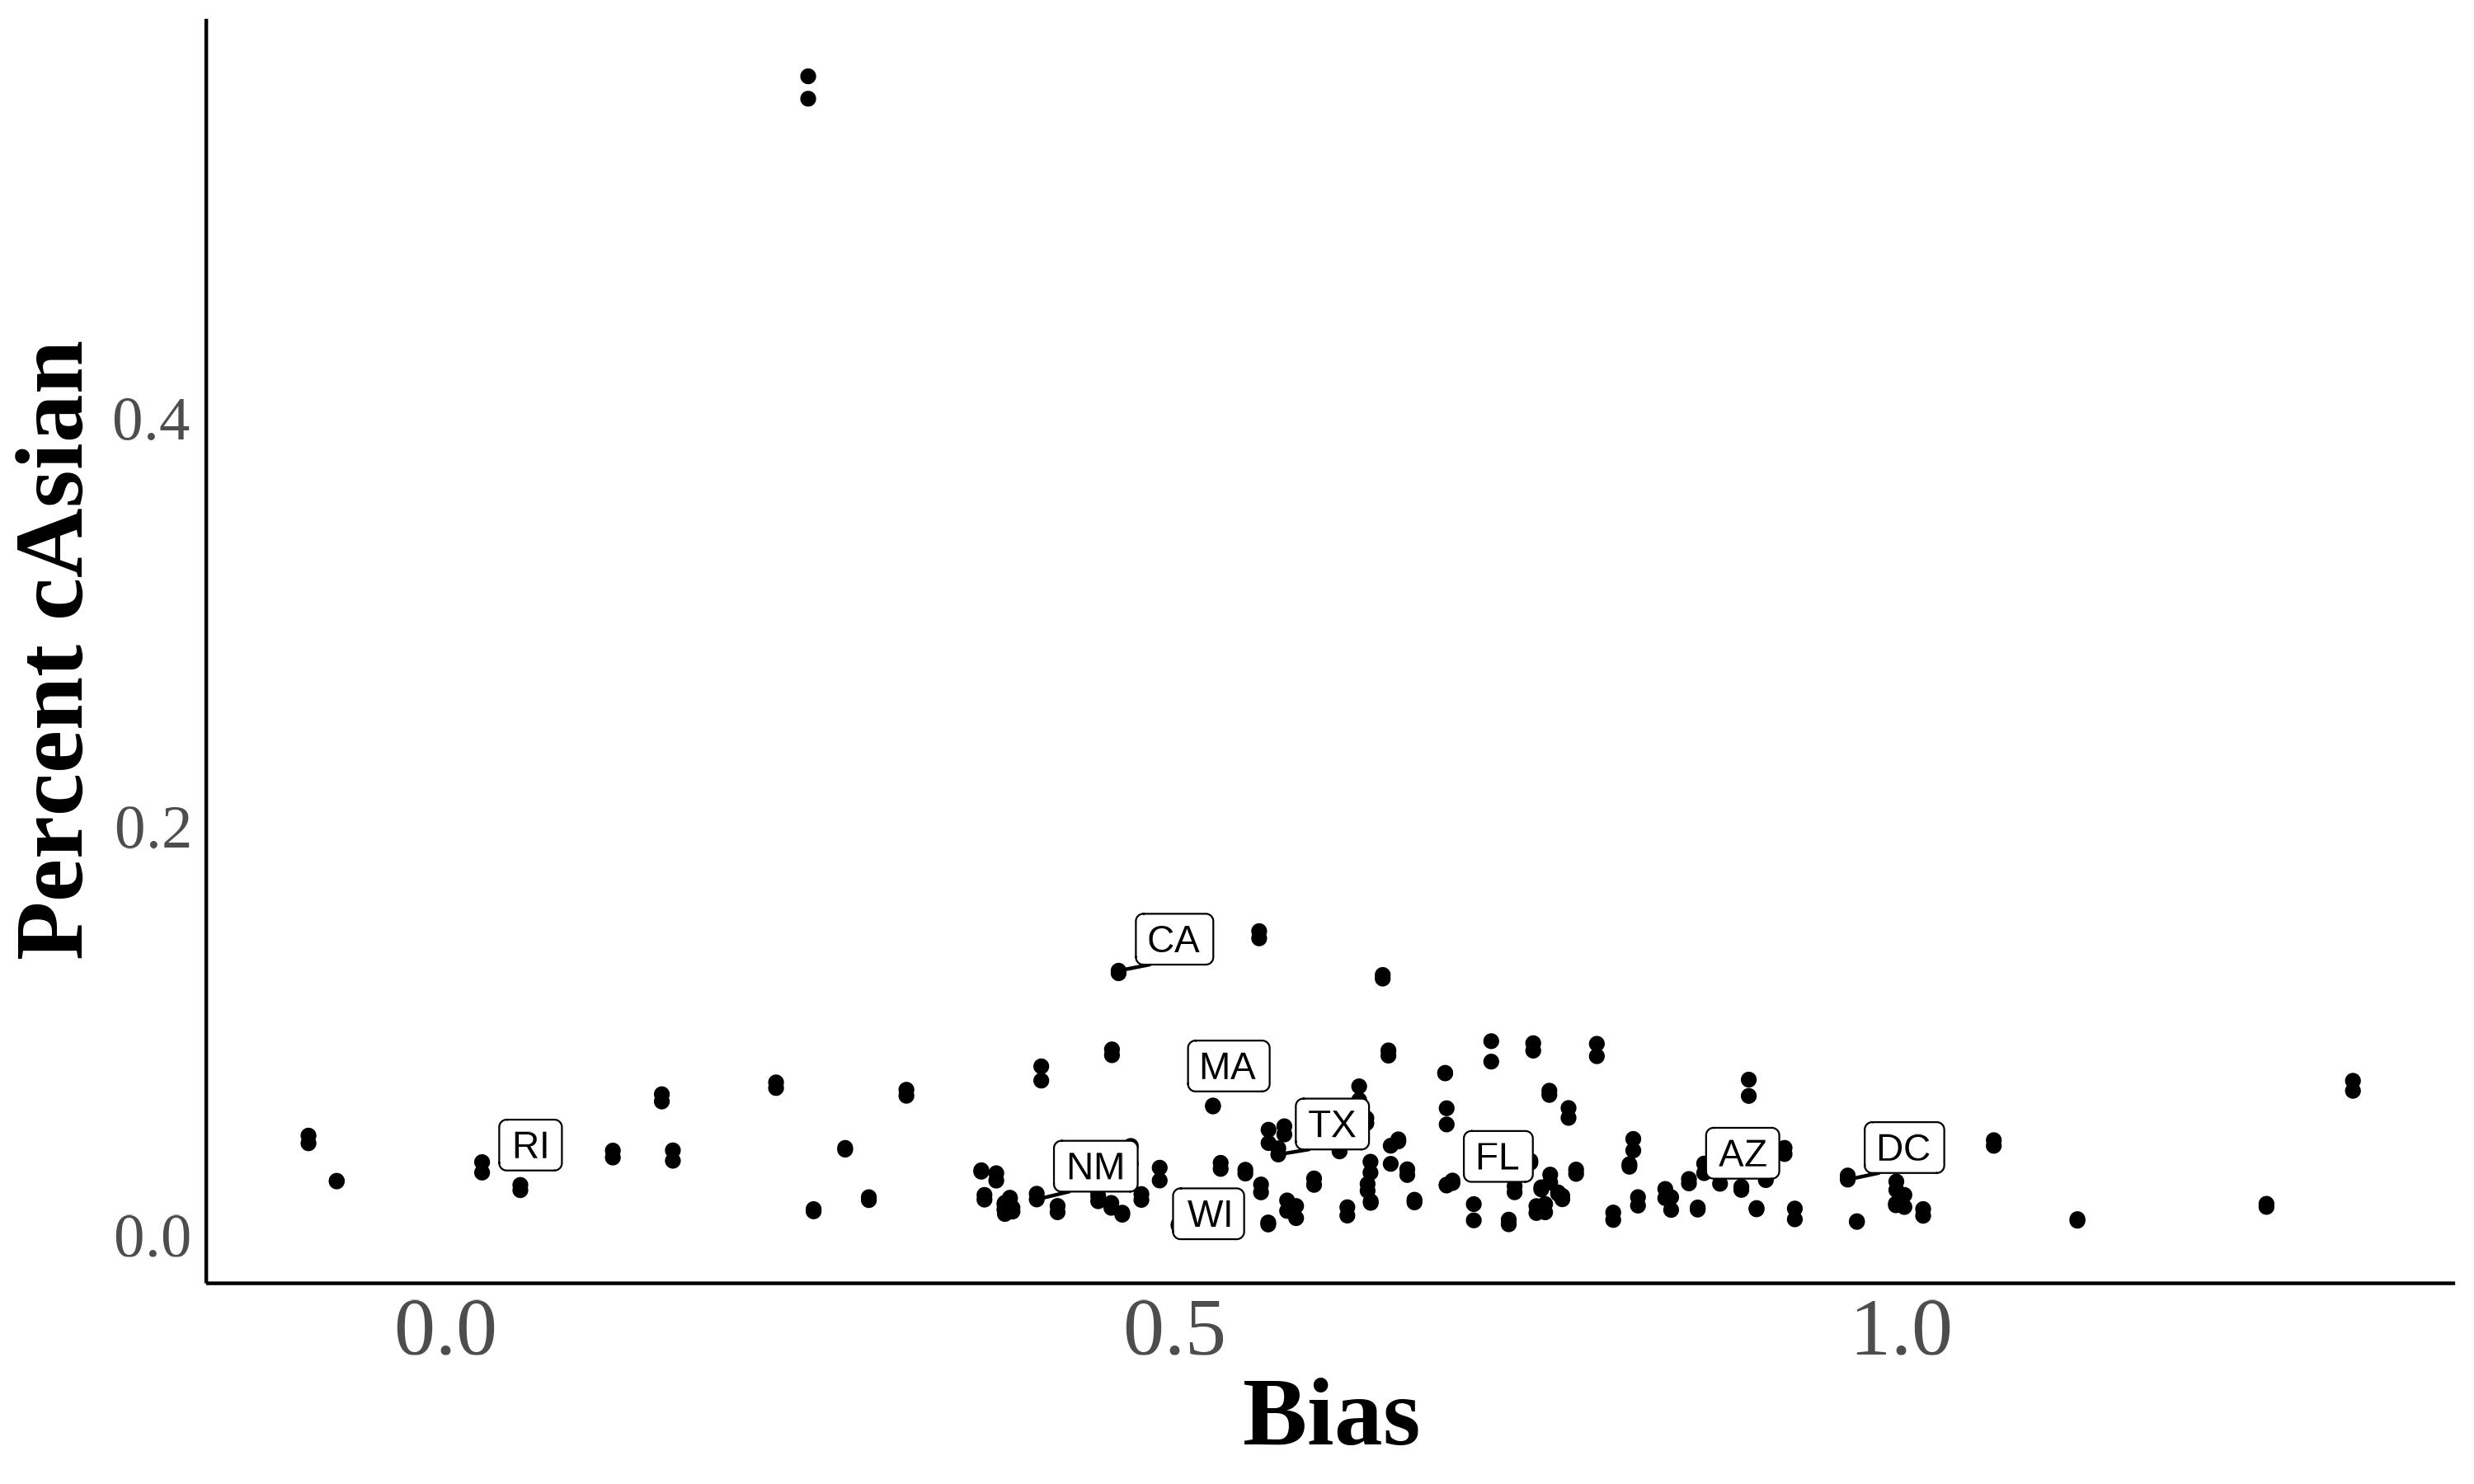
\includegraphics[width=.9\linewidth]{figure/scatter-plot-bias-Asian-less2015.png}
    \end{subfigure}
    \centering
    %Second graph
    \begin{subfigure}{.9\textwidth}
    \caption{Year $\geq$ 2015}
    \centering
    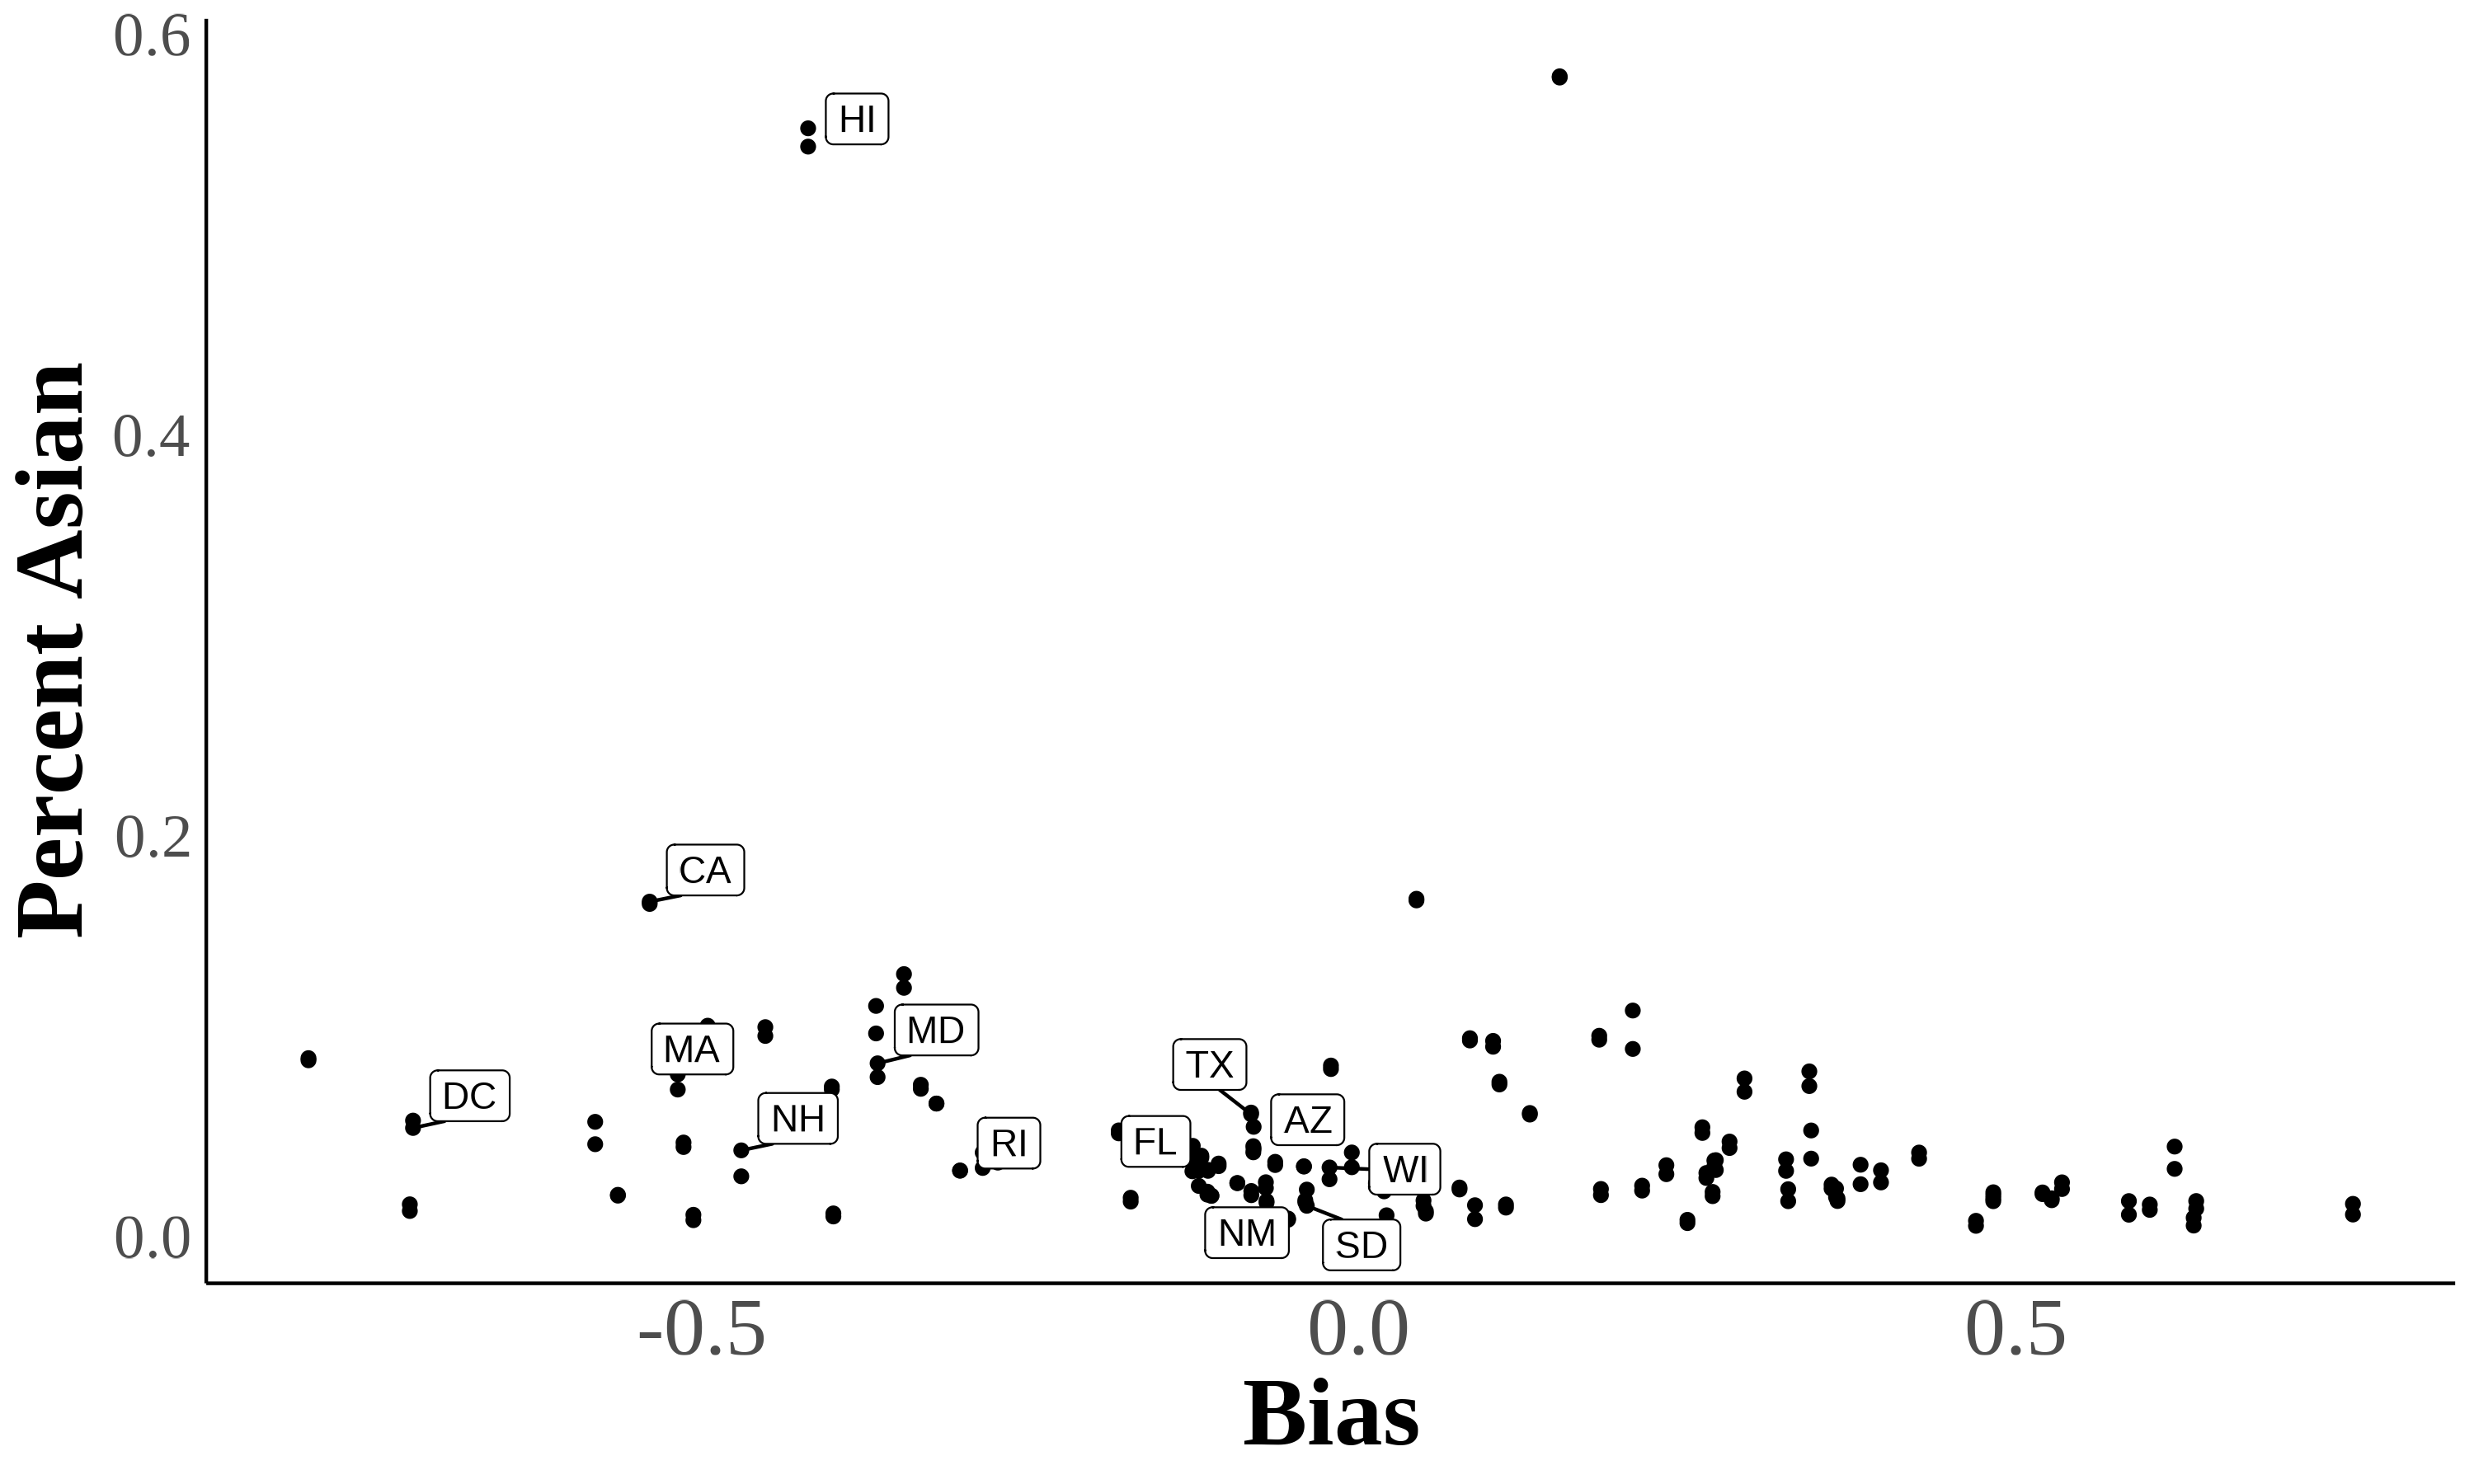
\includegraphics[width=.9\linewidth]{figure/scatter-plot-bias-Asian-great2015.png}
    \end{subfigure}
    \caption*{\footnotesize{Here are two scatter plots showing the relationship between bias and subjective Asian population in a state. Each dot represents a state in a certain year. Percent subjectively Asian = $\frac{\# \text{Asian}}{\text{Population}}$ \\
    \emph{Source.} 2004-2021 Current Population Survey.}}
    \end{figure}
    
\subsection{Using \textcite{lubotskyInterpretationRegressionsMultiple2006} to Construct Bias Index} % (fold)
\label{sub:lw-bias}
\begin{myRaggedRight}
In \textcite{lubotskyInterpretationRegressionsMultiple2006}, the authors propose a method to reduce measurement error in proxies by constructing a composite index. The Lubotsky-Wittenberg (henceforth LW) consider a model where a covariate is unobserved. Therefore, they use two proxies in its place, which will have measurement error. Thus, the LW method allows researchers to use two proxies that are error-ridden. 

LW consider a setup with the following model:

\begin{align*}
    y &= \alpha + \beta x^* + \epsilon \\
    x_1 &= x^* + \mu_1 \\
    x_2 &= x^* + \mu_2
\end{align*}

Where \(x_{i}^{*}\) is the unobserved covariate, \(x_{1i}\) and \(x_{2i}\) are the proxies, and the measurement errors \(\mu_1\) and \(\mu_2\) are assumed to be classical and allowed to covary. The covariance matrix of the errors is given by:

\[
\Sigma = \begin{bmatrix}
    \sigma_1^2 & \sigma_{12} \\
    \sigma_{12} & \sigma_2^2
\end{bmatrix}
\]

Replacing the unobserved \(x^*\) with \(x_1\) or \(x_2\) yields the following expectations of the OLS estimates:

\[
\mathbb{E} \left[ \hat{\beta}_1 \right] = \beta \frac{\sigma_{x^*}^2}{\sigma_{x^*}^2 + \sigma_1^2} \quad ; \quad \mathbb{E} \left[ \hat{\beta}_2 \right] = \beta \frac{\sigma_{x^*}^2}{\sigma_{x^*}^2 + \sigma_2^2}
\]

Both estimates are biased; the one with the smaller variance of the measurement error being less biased.

LW then propose defining a new proxy \(x_3\) as a weighted average of \(x_1\) and \(x_2\):

\[
x_3 = \lambda x_1 + (1 - \lambda) x_2
\]

To minimize the attenuation bias in the OLS estimate of \(\beta\), they solve for the optimal value of \(\lambda\):

\[
\lambda^* = \frac{\sigma_2^2 - \sigma_{12}}{\sigma_1^2 + \sigma_2^2 - 2\sigma_{12}}
\]

This optimal value of \(\lambda\) is not directly useful because the variances of the measurement errors and their covariance are unobserved. However, if you estimate a bivariate regression using OLS (i.e., regress \(y\) on \(x_1\) and \(x_2\)), then the expectation of the sum of the two coefficient estimates is identical to the expectation of the OLS coefficient estimate on \(x_3\) in a univariate regression using the optimal choice of \(\lambda\):

\[
\mathbb{E} \left[ \hat{\beta}_1 + \hat{\beta}_2 \right] = \mathbb{E} \left[ \hat{\beta}_{x_3} \right]
\]

Thus, OLS produces an estimate of \(\beta\) with the least bias by optimally combining the information in \(x_1\) and \(x_2\).
\end{myRaggedRight}
